\documentclass[two column, twoside, a4paper]{article}

\usepackage[utf8]{inputenc}
\usepackage{tcolorbox}
\usepackage[polish]{babel}
\usepackage[T1]{fontenc}
\usepackage[margin=0.5in]{geometry}
\usepackage[backend=biber, maxbibnames=4, style=authoryear, autocite=inline]{biblatex}
\usepackage{fancyhdr}
\usepackage{titlesec}
\usepackage{blindtext}

\addbibresource{$BIB}

\setlength{\columnsep}{1cm}

\title{Metody -omiczne, w badaniach wirusów}
\author{Jakub J. Guzek}
\date{}

% Section Formatting
\titleformat{\section}
{\sc \bfseries \Large}
{\thesection}
{0.5em}
{}[\titlerule]

\pagestyle{fancy}
\fancyhf{}
\fancyhead[RE, LO]{Szkoła Główna Gospodarstwa Wiejskiego}
\fancyhead[LE, RO]{Biotechnologia}
\fancyfoot[RE, LO]{Jakub J. Guzek}
\fancyfoot[LE, RO]{\thepage}
\fancyfoot[CE,CO]{Metody -omiczne, w badaniach wirusów}
\renewcommand{\footrulewidth}{0.05pt}

\begin{document}

\maketitle

\section{Wstęp}

Biologia molekularna jest jedną z najszybciej rozwijających się dziedzin wśród nauk biologicznych. Jej metody umożliwiają w dniu dzisiejszym sekwencjonowanie całych genomów -- co kiedyś było niemożliwe, lub pochłaniało ogromne zasoby zarówno pieniężne jak i czasowe -- w stosunkowo niedługim czasie. W rozwoju tych metod pomogły badania prowadzone na bardzo wielu, różnych organizmach i wirusach. Największy postęp przyniosły ogromne projekty takie jak \textbf{Projekt Poznania Genomu Człowieka} (\textit{Human Genome Project}) \autocite{IHGSC2001}, poznanie genomu neandertalczyka \autocite{Prufer2014}, czy projekt poznania genomu jęczmienia \autocite{IBGSC2012}.

Jak wspomniano wyżej, dzisiejsze metody umożliwiają sekwencjonowanie całych genomów w stosunkowo niedługim czasie, a wraz z opracowywaniem metod sekwencjonowania trzeciej i czwartej generacji możliwe będzie sekwencjonowanie ich w czasie rzeczywistym \autocite{Brown2019}. Prócz tego mikromacierze, hybrydyzacja i chromatografia powinowactwa umożliwiają badanie transkryptów genów i tworzenie transkryptomów (zbiorów wszystkich cząsteczek RNA w komórce) oraz zestawu białek komórkowych zwanego proteomem. Daje to możliwości badania komórki i interakcji molekularnych jakie są w niej obecne i umożliwia rozwój takim dziedzinom jak biologia systemów i interaktomika. Temu wszystkiemu towarzyszy oczywiście doskonalenia narzędzi informatycznych używanych do badań z zakresu \textit{-omics}, którym zajmuje się bioinformatyka.

\begin{figure}
\begin{tcolorbox}[sharp corners]
	\centering
	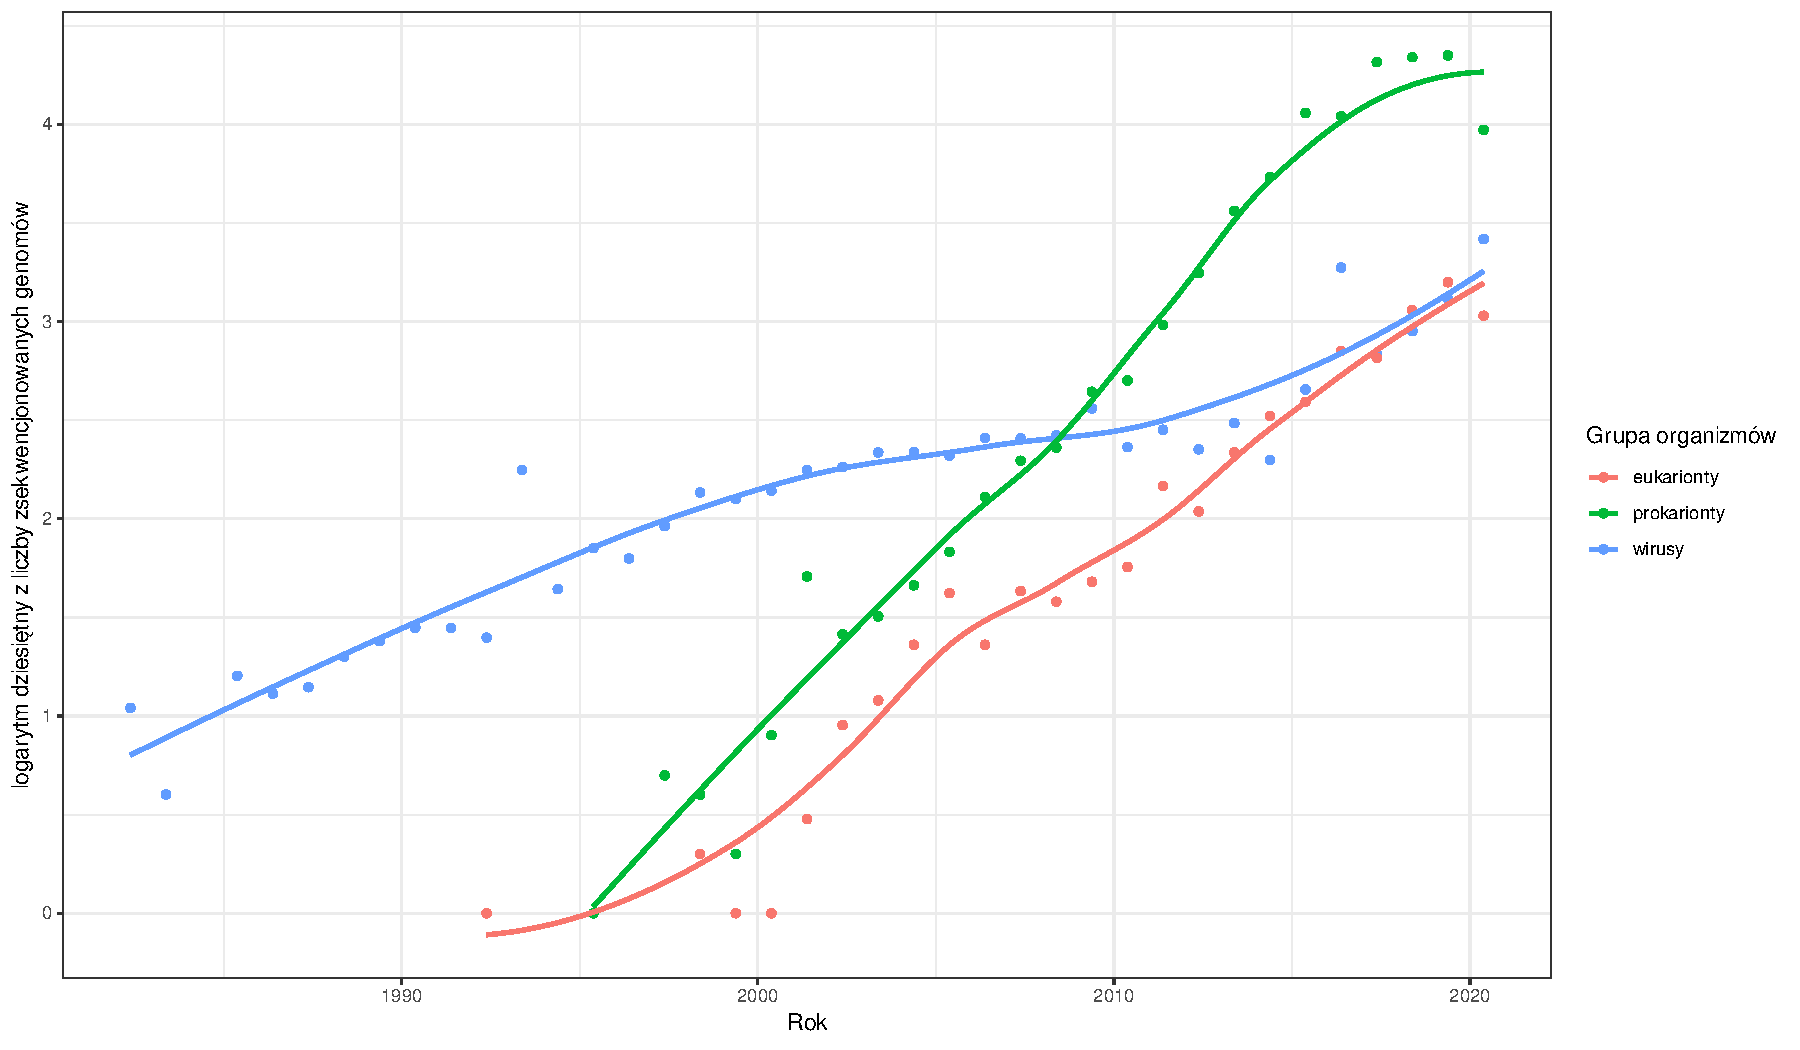
\includegraphics[width=\textwidth]{./sequenced_genomes.pdf}
	\caption{Ostatnie lata odnotowują bardzo szybki wzrost sekwencjonowanych genomów. Sekwencjonowanie genomów wirusowych odnotowuje jednak o wiele niższy wzrost niż prokariotycznych i eukariotycznych. Wykres przedstawia ilość genomów dodanych do bacy NCBI \autocite{NCBI} w danym roku.}\label{fig::seq_trends}

	\footnotetext{Autor pracy jest autorem wykresu, opracowanego na podstawie internetowej bazy danych NCBI. Kod wykresu można znaleźć pod adresem \textit{<++>}}
\end{tcolorbox}
\end{figure}

Które z tych metod są wykorzystywane w badaniu wirusów? Wiele z nich zostało opracowanych przy pracy na wirusach, zwłaszcza w początkowych dniach biologii molekularnej, gdy sekwencjonowanie genomów było przedsięwzięciem wielokrotnie trudniejszym niż dzisiaj, gdyż genomy wirusowe są niedużych rozmiarów, były więc atrakcyjnym materiałem badawczym. Wraz z postępem w tej dziedzinie wzrosła jednak ilość sekwencjonowanych genomów prokariotycznych i eukariotycznych (Rysunek \ref{fig::seq_trends}). Na dzień dzisiejszy w bazie danych NCBI jest ponad 30 tys. rekordów dla genomów wirusowych i ponad 200 tys. dla genomów prokariotycznych.

\printbibliography

\end{document}
